%% ****** Start of file apstemplate.tex ****** %
%%
%%
%%   This file is part of the APS files in the REVTeX 4 distribution.
%%   Version 4.1r of REVTeX, August 2010
%%
%%
%%   Copyright (c) 2001, 2009, 2010 The American Physical Society.
%%
%%   See the REVTeX 4 README file for restrictions and more information.
%%
%
% This is a template for producing manuscripts for use with REVTEX 4.0
% Copy this file to another name and then work on that file.
% That way, you always have this original template file to use.
%
% Group addresses by affiliation; use superscriptaddress for long
% author lists, or if there are many overlapping affiliations.
% For Phys. Rev. appearance, change preprint to twocolumn.
% Choose pra, prb, prc, prd, pre, prl, prstab, prstper, or rmp for journal
%  Add 'draft' option to mark overfull boxes with black boxes
%  Add 'showpacs' option to make PACS codes appear
%  Add 'showkeys' option to make keywords appear
\documentclass[aps,pre,reprint,superscriptaddress]{revtex4}
%\documentclass[aps,pre,preprint,superscriptaddress]{revtex4}
%\documentclass[aps,prl,reprint,groupedaddress]{revtex4}

% You should use BibTeX and apsrev.bst for references
% Choosing a journal automatically selects the correct APS
% BibTeX style file (bst file), so only uncomment the line
% below if necessary.
\bibliographystyle{apsrev4-1}

\usepackage{graphicx}
\usepackage{amsmath}

\newcommand{\e}[1]{\times10^{#1}}
\newcommand{\gd}{\dot{\gamma}}

\begin{document}

% Use the \preprint command to place your local institutional report
% number in the upper righthand corner of the title page in preprint mode.
% Multiple \preprint commands are allowed.
% Use the 'preprintnumbers' class option to override journal defaults
% to display numbers if necessary
%\preprint{}

%Title of paper
\title{Rheology of Cubic Blue Phases}

% repeat the \author .. \affiliation  etc. as needed
% \email, \thanks, \homepage, \altaffiliation all apply to the current
% author. Explanatory text should go in the []'s, actual e-mail
% address or url should go in the {}'s for \email and \homepage.
% Please use the appropriate macro foreach each type of information

% \affiliation command applies to all authors since the last
% \affiliation command. The \affiliation command should follow the
% other information
% \affiliation can be followed by \email, \homepage, \thanks as well.
\author{O. Henrich}
\email[Corresponding author: ]{o.henrich@ucl.ac.uk}
\affiliation{Edinburgh Parallel Computing Centre, School of Physics and Astronomy, University of Edinburgh, JCMB Kings Buildings, Mayfield Road, Edinburgh EH9 3JZ, UK}
\affiliation{Centre for Computational Science, University College London, 20 Gordon Street, London WC1H 0AJ, UK}

\author{K. Stratford}
\affiliation{Edinburgh Parallel Computing Centre, School of Physics and Astronomy, University of Edinburgh, JCMB Kings Buildings, Mayfield Road, Edinburgh EH9 3JZ, UK}

\author{P.V. Coveney}
\affiliation{Centre for Computational Science, University College London, 20 Gordon Street, London WC1H 0AJ, UK}

\author{M.E. Cates}
\affiliation{SUPA, School of Physics and Astronomy, University of Edinburgh, JCMB Kings Buildings, Mayfield Road, Edinburgh EH9 3JZ, UK}

\author{D. Marenduzzo}
\affiliation{SUPA, School of Physics and Astronomy, University of Edinburgh, JCMB Kings Buildings, Mayfield Road, Edinburgh EH9 3JZ, UK}

%\homepage[]{Your web page}
%\thanks{}
%\altaffiliation{}

%Collaboration name if desired (requires use of superscriptaddress
%option in \documentclass). \noaffiliation is required (may also be
%used with the \author command).
%\collaboration can be followed by \email, \homepage, \thanks as well.
%\collaboration{}

%\noaffiliation

\date{\today}

\begin{abstract}
We study the behaviour of cubic blue phases under shear flow
via lattice Boltzmann simulations. We focus on the two experimentally observed
phases, Blue Phase I (BPI) and Blue Phase II (BPII). The disclination network of Blue Phase 
II continuously breaks and reforms under shear, leading to an oscillatory stress response in time.
\end{abstract}

% insert suggested PACS numbers in braces on next line
\pacs{47.11.Qr, 47.57.Lj, 47.57.Qk, 61.30.Dk, 61.30.Pq, 61.30.Jf, 83.80.Xz}
% insert suggested keywords - APS authors don't need to do this
%\keywords{}

%\maketitle must follow title, authors, abstract, \pacs, and \keywords
\maketitle

% body of paper here - Use proper section commands
% References should be done using the \cite, \ref, and \label commands
\section{Introduction}
% Put \label in argument of \section for cross-referencing
%\section{\label{}}

Cholesterics are liquid crystals in which the local nematic director field spontaneously 
twists in thermodynamic equilibrium~\cite{deGennes}. The preferred configuration close 
to the isotropic boundary features twist around two perpendicular axes, as opposed to 
just one axis in the regular cholesteric state, and the corresponding deformation is 
denoted a ``double-twist cylinder''.
As it is topologically impossible to cover continuously 3D space with double-twist 
cylinders, defects arise. These organise into a variety of regular periodic lattices, 
giving rise to the so-called cubic blue phases (BPs)~\cite{Grebel:1984,Wright:1989}. 
There are two experimentally observed cubic blue phases, BPI and BPII (a third, BPIII, 
is thought to be amorphous~\cite{Henrich:2011a}).

BPs have been long considered as purely of academic interest due to their very narrow 
range of stability. This view has changed since the creation of polymer-stabilised and 
temperature-stabilised BPs~\cite{Kikuchi:2002,Coles:2005}, which has opened up the 
possibility of novel applications.
During the last few years considerable progress has been achieved regarding the behaviour 
of BPs in confined geometries~\cite{Fukuda:2010a, Fukuda:2010b, Ravnik:2011b}, under 
external fields ~\cite{Alexander:2008,Fukuda:2009,Henrich:2010a,Castles:2010,Tiribocchi:2011a}, 
and in the presence of colloidal particles~\cite{Ravnik:2011a}.
The kinetics of BP domain growth have been recently addressed in~\cite{Henrich:2010b}. 
However, our understanding of their dynamical behaviour under flow remains
very limited. The aim of this work is to address this issue by studying,
for the first time, the response of confined BP samples to a shear flow.

Flow response in cholesterics is both strongly non-Newtonian and highly anisotropic.
For example, if a cholesteric helix is subjected to a Poiseuille flow along
the helical axis, small pressure differences drive flow mainly through
``permeation'', first investigated by Helfrich~\cite{Helfrich:1969}.
In the permeation mode the liquid crystal flows while leaving the director
field virtually unchanged, which leads to high dissipation and large
viscosities. Marenduzzo et al.~\cite{Marenduzzo:2006a,Marenduzzo:2006b} simulated 
shear and Poiseuille flow in cholesteric liquid crystals in the permeation mode, and 
showed the importance of the boundary conditions in determining the apparent viscosity of the fluid. 
They also found that a strong secondary flow appears.
Rey~\cite{Rey:1996a, Rey:1996b} studied shear in cholesterics oriented with the helix along 
the vorticity axis and found that, at low Ericksen number, travelling twist waves appear which 
lead to the rotation of the cholesteric helix. At higher forcing, the helix uncoils and 
leaves a flow-induced nematic phase.
Rey also studied cholesterics subjected to both steady flow and low frequency
small amplitude oscillatory shear for different helix orientations
~\cite{Rey:2000, Rey:2002}. He found that splay/bend/twist deformations were
excited when the helix was aligned along the flow direction; splay/bend
deformation occurred when the helix was aligned along the velocity gradient;
but only twist deformations
appeared when the helix was aligned along the vorticity axis.

Dupuis et al.~\cite{Dupuis:2005} performed the first numerical investigation of BP rheology 
in Poiseuille flow, starting from equilibrium structures of BPI and BPII and a periodic 
array of doubly twisted cylinders.
Under small forcing, the network opposed the flow giving rise to a significant 
increase in apparent viscosity.
Upon increasing the forcing they found clear evidence of shear thinning.
In the crossover region they predicted a novel oscillatory regime where the network 
continuously breaks and reforms as portions of the disclinations in the center of the channel 
move to neighboring cells and relink with the parts of the network left behind by the flow. 
Compared with the cholesteric case, the viscosity still decreases with forcing 
(the system shear thins) but much less than
for cholesterics in the permeation mode, which is in agreement with experiments
~\cite{Zapotocky:1999, Ramos:2002}.

\section{Model and Methods}

Our approach is based on the well-established Beris-Edwards model for hydrodynamics of
cholesteric liquid crystals \cite{Beris:1994}, which describes the ordered state 
in terms of a traceless, symmetric tensor order parameter ${\mathbf Q}({\mathbf r})$. 
In the uniaxial approximation, the order parameter is given by
$Q_{\alpha \beta}= q_s ( n_\alpha n_\beta - \frac{1}{3}\; \delta_{\alpha\beta})$
with ${\mathbf n}$ the director field and $q_s$ the amplitude of nematic
order. More generally,
the largest eigenvalue of ${\mathbf Q}$, $0\le q_s\le\frac{2}{3}$
characterizes the local degree of orientational order.
The thermodynamic properties of the liquid crystal are determined by a free energy
${\cal F}$, whose density $f$ consists of a bulk contribution $f_b$ and a gradient part $f_g$, as follows,
\begin{eqnarray}
f_b&=&\frac{A_0}{2}\left(1-\frac{\gamma}{3}\right) Q_{\alpha \beta}^2-\frac{A_0 \gamma}{3}Q_{\alpha \beta} Q_{\beta \gamma} Q_{\gamma \alpha}+\frac{A_0 \gamma}{4}(Q_{\alpha \beta}^2)^2,\nonumber\\
f_g&=&\frac{K}{2}(\varepsilon_{\alpha\gamma\delta} \partial_\gamma Q_{\delta\beta}+2 q_0 Q_{\alpha \beta})^2+\frac{K}{2}(\partial_\beta Q_{\alpha \beta})^2.\label{FE}
\end{eqnarray}
The first term contains the bulk-free energy constant $A_0$ and the inverse temperature $\gamma$ which controls the magnitude of order.
The second part quantifies the cost of elastic distortions, which are proportional to the elastic constant $K$;
we work for simplicity in the one-elastic constant approximation. The wavevector $q_0=2\pi/p_0$, where $p_0$ is the cholesteric pitch.
The actual periodicity of the BP structure, $p$, does not need to be equal to $p_0$.
The ``redshift'' $r=p/p_0$ is adjusted during the simulation by following a simple procedure similar to~\cite{Alexander:2006}.

A particular thermodynamic state is specified by two dimensionless quantities: the effective temperature $\tau$ and chirality $\kappa$,
which are given by
\begin{eqnarray}
\tau&=&\frac{27(1-\gamma/3)}{\gamma}\nonumber\\
\kappa&=&\sqrt{\frac{108 K q_0^2}{A_0 \gamma}}\nonumber.
\end{eqnarray}
The dynamical evolution of the order parameter is given by the equation 
\begin{equation}
\left(\partial_t+ u_\alpha \partial_\alpha \right){\mathbf Q} - {\mathbf S}({\mathbf W},{\mathbf Q}) = \Gamma {\mathbf H}.
\label{eqn2}
\end{equation}
The first term on the left hand side of Eq.\ref{eqn2} is a material derivative, which describes the rate of change of a quantity moving along with the flow.
The second term accounts for the rate of change due to local velocity gradients $W_{\alpha \beta}=\partial_\beta u_\alpha$,
\begin{eqnarray}
{\mathbf S}({\mathbf W}, {\mathbf Q}) &=& (\xi {\mathbf A} + {\boldsymbol \Omega})({\mathbf Q}+\frac{\mathbf I}{3})\nonumber\\
& &\hspace*{-1.5cm}+ ({\mathbf Q}+\frac{\mathbf I}{3})(\xi {\mathbf A}  - {\boldsymbol \Omega})-2 \xi ({\mathbf Q}+\frac{\mathbf I}{3})
\mathrm{Tr}({\mathbf Q W}),
\label{eqn3}
\end{eqnarray}
where $\mathrm{Tr}$ denotes the tensorial trace, while 
${\mathbf A}=({\mathbf W}+{\mathbf W}^T)/2$ and
${\boldsymbol \Omega}=({\mathbf W}-{\mathbf W}^T)/2$ are the symmetric and antisymmetric part of the velocity gradient, respectively. $\xi$ 
is a constant depending on the molecular details of the liquid crystal.
Flow alignment occurs if $\xi \cos{2\theta}=(3q_s)/(2+q_s)$ has a real solution, where $\theta$ is the Leslie-angle: we select this case by 
setting $\xi=0.7$ in our simulations.
${\mathbf H}$ is the molecular field, which is a functional derivative of $\cal F$ that preserves the tracelessness of $\mathbf Q$:
\begin{equation}
{\bf H}=-\frac{\delta {\cal F}}{\delta {\bf Q}}+\frac{\bf I}{3}\,
\mathrm{Tr} \left(\frac{\delta {\cal F}}{\delta {\bf Q}}\right).
\label{eqn4}
\end{equation}
The rotational diffusion constant $\Gamma$ in Eq.~\ref{eqn2} is proportional
to the inverse of the rotational viscosity $\gamma_1=2 q_s^2/\Gamma$
\cite{deGennes}.

The time evolution of the fluid density and velocity are respectively governed
by the continuity equation
$\partial_t \rho = -\partial_\alpha(\rho u_\alpha)$, and
the following Navier-Stokes equation:
\begin{eqnarray}
\partial_t u_\alpha +\rho \,u_\beta \partial_\beta u_\alpha
= \partial_\beta \Pi_{\alpha \beta}
+\eta\, \partial_\beta \{ \partial_\alpha u_\beta + \partial_\beta u_\alpha
+(1+3\frac{\partial P_0}{\partial\rho} )\partial_\mu u_\mu \delta_{\alpha \beta}\}. 
\label{eqn6}
\end{eqnarray}
The final term in Eq.~\ref{eqn6} arises from the Chapman-Enskog expansion
of the LB equations \cite{Denniston:2001}.
At low flow rates the fluid can be considered as incompressible, so that the
last term on the right hand side of Eq.~\ref{eqn6} remains small.
$\eta$ is an isotropic background viscosity which is set to $\eta=0.8333$ in LBU.
The pressure tensor reads explicitly
\begin{eqnarray}
\Pi_{\alpha \beta}&=&P_0 \delta_{\alpha\beta}
-\xi H_{\alpha \gamma}\left(Q_{\gamma \beta} +\frac{1}{3} \delta_{\gamma \beta}\right)-\xi \left(Q_{\alpha \gamma} +\frac{1}{3} \delta_{\alpha \gamma}\right) H_{\gamma \beta}\nonumber\\
&+& 2 \xi  \left(Q_{\alpha \beta} +\frac{1}{3} \delta_{\alpha \beta}\right) Q_{\gamma \nu} H_{\gamma \nu}-\partial_\alpha Q_{\gamma \nu} \frac{\delta{\cal F}}{\delta \partial_{\beta} Q_{\gamma \nu}}\nonumber\\
&+&Q_{\alpha \gamma}H_{\gamma \beta}-H_{\alpha \gamma} Q_{\gamma \beta}.
\label{eqn7}
\end{eqnarray}
In the isotropic state ${\bf Q}\equiv 0$ and Eq.\ref{eqn7} is reduced to the
scalar pressure which, in a system at rest, is constant to a very good
approximation.
 
The system of coupled partial differential equations Eqs.~\ref{eqn2}
and~\ref{eqn6} is solved by means of a
hybrid scheme~\cite{Marenduzzo:2007}. This uses a lattice Boltzmann algorithm
with predictor-corrector scheme for the continuity equation and
Eq.~\ref{eqn6}, and a finite difference scheme for the equation of motion of
the tensor order parameter Eq.\ref{eqn2}. More details on the algorithm can
be found in~\cite{Denniston:2001, Denniston:2004}.

\section{Results and Discussion}

In the following we report results of simulations of the bulk flow behaviour of the cubic blue 
phases BPI and BPII. The thermodynamic states are characterised by an effective temperature 
$\tau$ and the chirality $\kappa$, which measures the ratio of gradient to bulk free energy terms.
We opted for states sufficiently far away from the chiral-nematic-isotropic 
where both quiescent blue phases are at equilibrium, namely
$\tau=-0.5, \kappa=1.0$ in case of BPI and $\tau=-0.5, \kappa=2.0$ (BPII), respectively.
Simulations at metastable states at higher and lower temperatures and different chiralities showed 
no differences in their generic flow behaviour.
However, states closer to the phase boundary featuring higher free energy densities and 
smaller average order parameters show a tendency to break up more easily under external driving forces.

As is common in BP simulation studies~\cite{Henrich:2011a,Henrich:2010b}, we initialised our simulations with 
analytical solutions that minimize the free energy functional Eq.\ref{FE} in the high-chirality limit, 
and equilibrated these (for 5000 LB timesteps) prior to starting the shear. 
During the equilibration run the optimal redshift $r$ was recalculated at every timestep.
After equilibration the redshift parameter was kept constant throughout the rest of the simulation.
We chose a unit cell size of 16 lattice sites for BPII and 32 sites in case of BPI. 
Runs with higher resolution confirmed that this was an appropriate minimal resolution to cover 
the complex conformational changes and kinematic details of the blue phase networks.

Simple shear flow is imposed by means of a Lees-Edwards boundary condition ~\cite{Wagner:2002} with
the top (bottom) half of the planes moving in positive (negative) x-direction.
We applied a correction for spurious momentum currents that emerge due to interpolations accross 
the Lees-Edwards planes \cite{Henrich:2012a}.
The shear rates were varied over more than two orders of magnitude from about 
$\gd=2.44\times \e{-6}$ to $6.3\times\e{-4}$ in LB units.
The shear flow was imposed along the x-axis, whereas velocity gradient and vorticity are oriented 
along the y- and z-axis.
Disclination lines are plotted as isosurface of the scalar order parameter $q$. Typical values 
are $q_s=0.18$ for BPI and $q_s=0.15$ for BPII.
The timestep and lattice spacing in lattice Boltzmann units (LBU) corresponds roughly to
$\sim 1 {\rm ns}$ and $\sim 10{\rm nm}$ in SI units. The LBU of stress
is equal to about $10^8$~Pa.
More details about the conversion from LBU to SI units can be found in
\cite{Henrich:2011a,Henrich:2010b}.

\subsection{Blue Phase II}

We start the discussion with BPII. Fig \ref{bp2-med} shows the disclination network 
undergoing an affine transformation under shear. The disclination lines break up and 
reconnect further downstream forming a periodically recurring pattern. 
Apart from the affine transformation the general appearance is very close to that 
of the quiescent equilibrium phase.

\begin{figure*}[h]
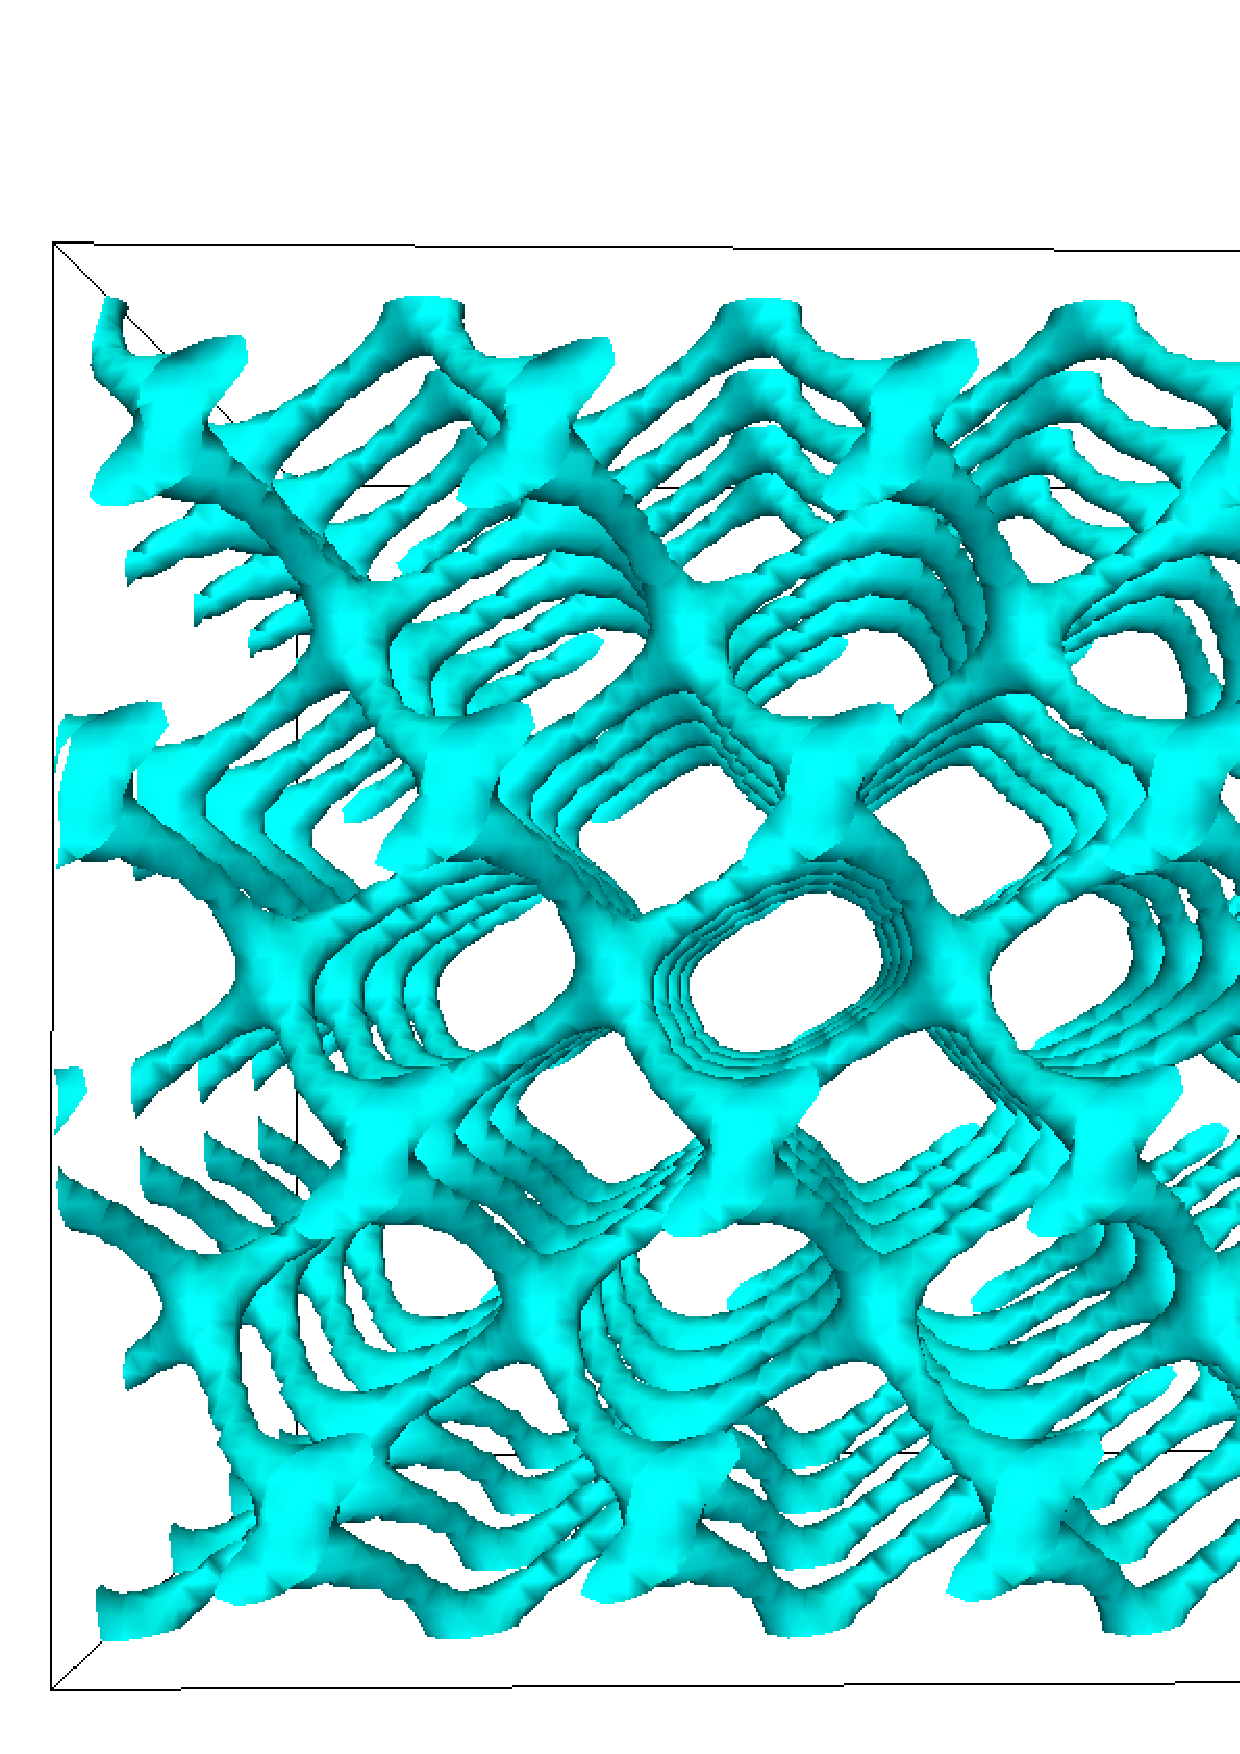
\includegraphics[width=0.32\textwidth]{disc-160k_run902.png}
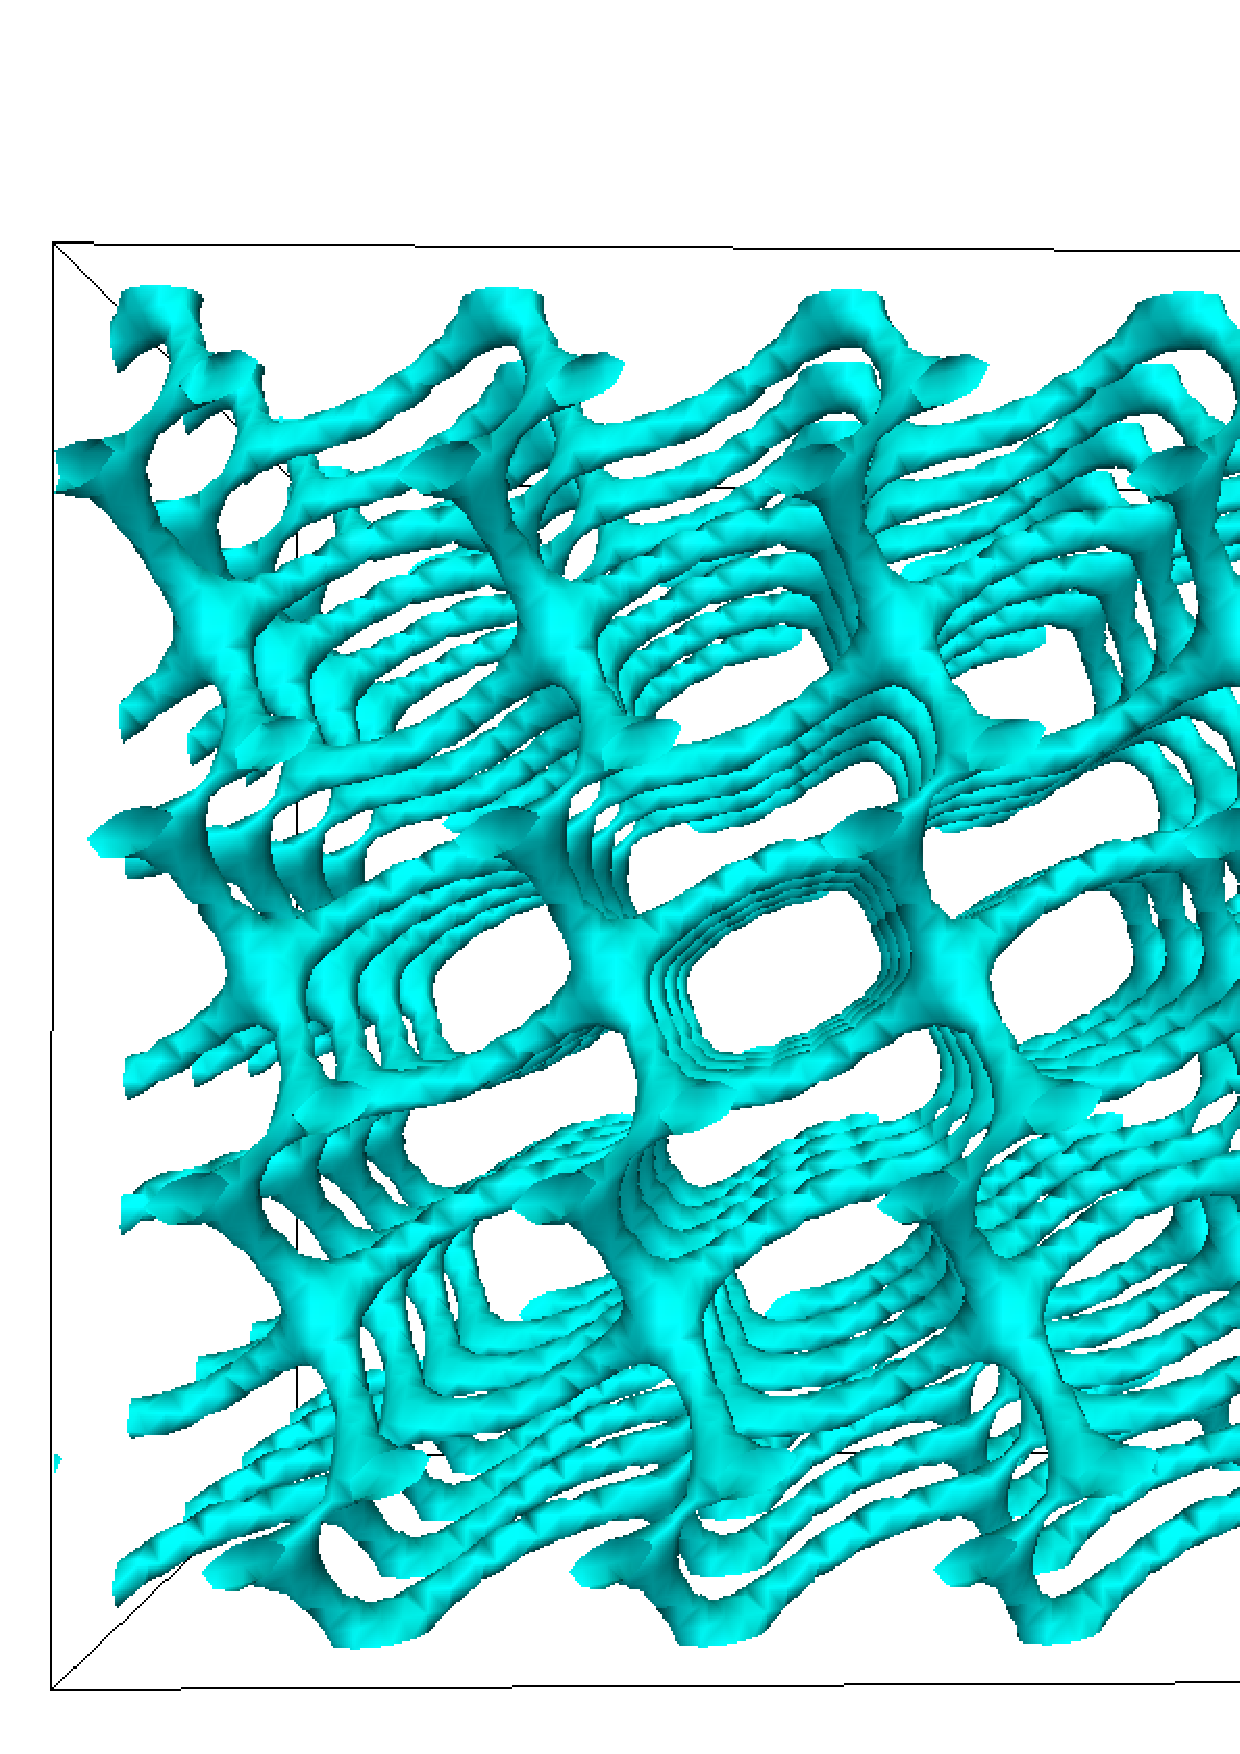
\includegraphics[width=0.32\textwidth]{disc-164k_run902.png}
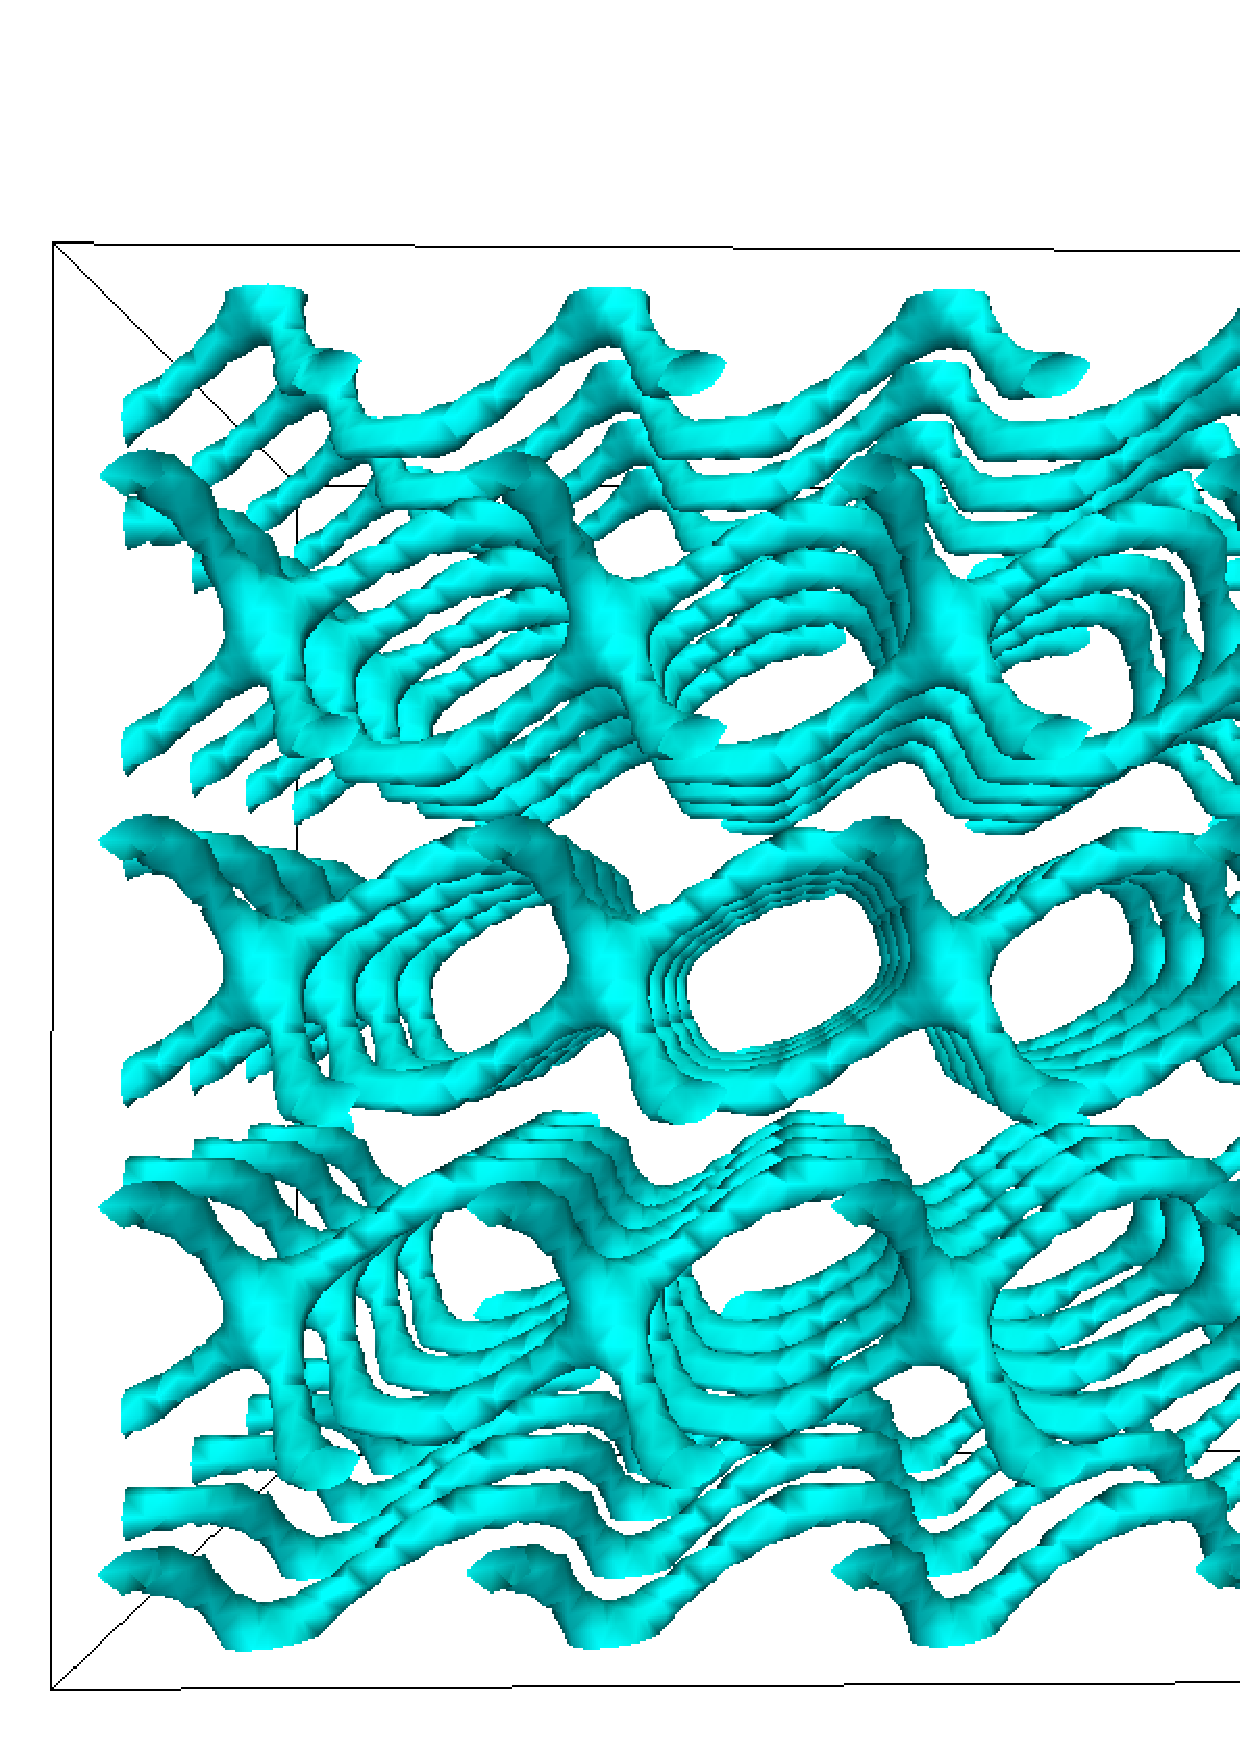
\includegraphics[width=0.32\textwidth]{disc-165k_run902.png}
\caption{Disclination network of BPII in shear flow: The pictures show a typical sequence 
of shear-induced transformations in the steady state at 
$\gd=1.56\e{-4}$ and time steps $t=1.60, 1.64,1.65\e{5}$. The velocity gradient 
is oriented along the vertical direction, whereas the horizontal direction is the direction of flow. 
The boundary conditions are applied flow takes place in such as way that network moves 
to the right in the upper half and to the left in the lower half.}
\label{bp2-med}
\end{figure*}

Interestingly, while being sheared the disclination network moves perpendicular to the flow and 
the gradient direction in the direction of vorticity.
Contrary to the stick-slip motion that has been observed for sheared blue phases in confined
geometries~\cite{Henrich:2012b} the movement is steady and happens in such a way that the 
positions of breakup and reconnection shown in Fig. \ref{bp2-med} are slightly offset, 
making the network travel along the z-direction.
The recurrence period in vorticity direction is exactly six times larger than that of reconnecting in flow direction.

Fig. \ref{bp2-velo} shows the disclination network at a characteristic time step between reconnecting and another breakup.
Superimposed are vectors which represent the velocity projected onto a plain perpendicular to the flow direction.
This projection makes it possible to get rid of the dominating velocity component $v_x$ and permits visualisation the 
two much smaller components $v_y$ and $v_z$.
The magnitude of the minor components is typically in the range of a few percent of the primary flow component.
Characteristic bands oriented along the vorticity direction form, which are normally hidden behind the primary flow in x-direction.
When the helicity of the underlying cholesteric phase is changed from a left- to a righthanded helix the sign of $v_z$ 
and the sense of motion also changes.
Further quantitative evidence for a direct link between flow direction and helicity can be found by time-averaging over
individual cycles.
Tab. \ref{tab1} gives minima, maxima, averages and standard deviations of the velocity components.
All values for the two runs with inverted helicity are identical apart from a change of sign in the z-components.
There is only a slight imbalance between the maximum and minimum velocity in z-direction.
Hence the movement of the network in vorticity direction is predominantly permeative.
Note that the imbalance is exaclty retained if the helicity is inverted.

\begin{figure*}[h]
\includegraphics[width=0.495\textwidth]{v_yz-v_z-160k_run902.png}
\includegraphics[width=0.495\textwidth]{v_yz-v_z-160k_run903.png}
\caption{Velocity patterns and disclination network in BPII for positive (left) and negative (right) helicity of the 
underlying cholesteric helix: The pictures show velocity vectors $(0,v_y,v_z)$ in x-direction, 
i.e. the velocity has been projected onto a plane perpendicular to the flow direction. 
The vertical and horizontal direction are the gradient and vorticity direction, respectively.
The colour code gives the magnitude and sign of the component in vorticity direction.
The snapshot shows a typical frame during a periodically recurring sequence.
The network on the left with positive helicity travels rightwards, whereas the one one the right
moves leftwards. The recurrence period in vorticity direction is six times longer than the time it takes the network 
to reconnect in flow direction.}
\label{bp2-velo}
\end{figure*}

If the flow rate exceeds a certain critical value BPII ceases to undergo the affine transformation under shear that we
descibed above. Fig. \ref{bp2-high} shows a cut through the director field of BPII at high shear rate.
The entire blue phase network has breaken up into a simple cholesteric phase. The preferred mode of flow is 
a travelling helical wave with the helical axis oriented along the vorticity direction and translational 
invariance in flow and gradient direction. This mode of flow is the preferred one for low Ericksen numbers
before a helix uncoiling transition to a nematic flow aligned state takes place at even higher
shear rates \cite{Rey:1996a, Rey:1996b}.

In our scenario the break-up occurs for shear rates between $\gd=3.12\e{-4}$ and $6.25\e{-4}$.
However, it is reasonable to assume that the critical shear rate depends on thermodynamic and kinetic parameters
such as the effective temperature $\tau$, the chirality $\kappa$ and the rotational diffusion constant $\Gamma$.
Due to a lack of computational resources we have not investigated these aspects any further.

\begin{figure}[h]
\includegraphics[width=0.85\textwidth]{dir+y-250k_run949.png}
\includegraphics[width=0.85\textwidth]{dir+y-253k_run949.png}
\includegraphics[width=0.85\textwidth]{dir+y-255k_run949.png}
\includegraphics[width=0.85\textwidth]{dir+y-257k_run949.png}
\caption{Director field of BPII at high shear rate: The images show a sequence of time step $t=2.50, 2.53,2.55, 2.57\e{5}$ (from top to bottom). The images show 1D-cuts as the configuration is translationally invariant in flow and gradient direction. The configuration is a travelling helical wave along the vorticity or z-direction. The colour code indicates the orientation in x-y direction.}
\label{bp2-high}
\end{figure}

A quantitative analysis of the flow behaviour of BPII is shown in Fig. \ref{bp2-rheo}.
The apparent viscosity $\eta_{app}=\Pi_{xy}/\eta\,\gd$ over time normalised to
the isotropic background viscosity $\eta_{app}$ is given in the left image, whereas
the picture on the right shows the same data versus accummulated total strain.
For all but the highest flow rates $\eta_{app}$ oscillates sinusoidally, which
is due to the periodic break-up and reconnection of the network under shear flow.

The inset shows the time average of the deviatoric part of the stress tensor $\bar{Pi}_{xy}$ as a function of shear rate.
The error bars indicate the maximum and minimum stresses that occur during one cycle.
The data for low and intermediate $\gd$ obeys a power law fit $\bar{\Pi}_{xy}=a \gd^b$ with $a=0.34(99), b=0.95(38)$ to
a very good approximation, exibiting a remarkably small degree of shear-thinning.
This probably reflects the very regular and rather undisturbed affine transformation of the disclination network.  

\begin{figure*}[h]
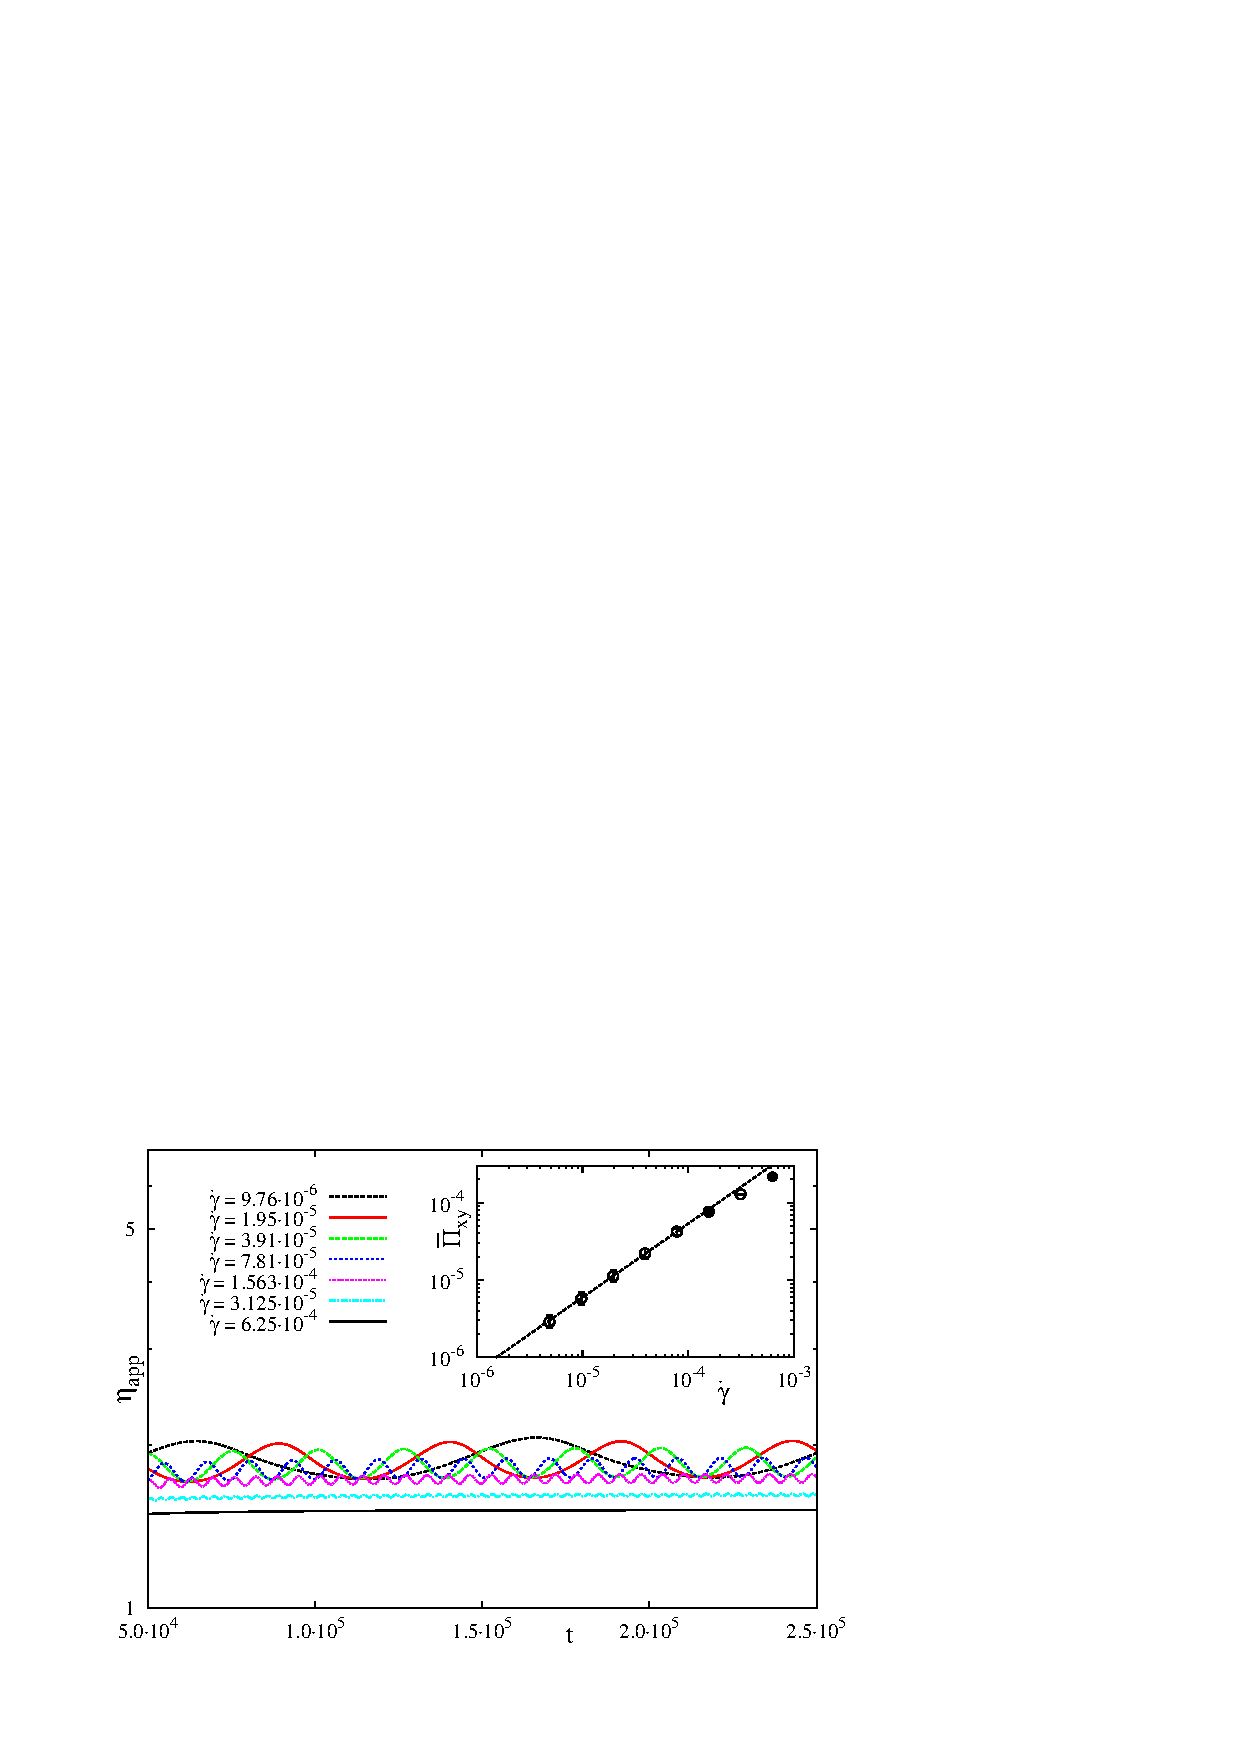
\includegraphics[width=0.495\textwidth]{stress_bp2.pdf}
\includegraphics[width=0.495\textwidth]{stress_vs_strain_bp2.pdf}
\caption{Apparent viscosity $\eta_{app}=\Pi_{xy}/\eta\,\gd$ of BPII over time (left) and strain (right). The inset shows the flow curve $\bar{\Pi}_{xy}(\gd)$.}
\label{bp2-rheo}
\end{figure*}

\clearpage

\subsection{Blue Phase I}



The flow behaviour of BPI at low shear rates is is similar deviates significantly from that of BPII in a number of points.

\begin{figure}[h]
\includegraphics[width=0.32\textwidth]{disc-xy-400k_run1115.png}
\includegraphics[width=0.32\textwidth]{disc-yz-400k_run1115.png}
\includegraphics[width=0.32\textwidth]{disc-xy-600k_run1115.png}\\
\includegraphics[width=0.32\textwidth]{disc-xy-725k_run1115.png}
\includegraphics[width=0.32\textwidth]{disc-xy-750k_run1115.png}
\includegraphics[width=0.32\textwidth]{disc-xy-775k_run1115.png}
\caption{Disclination network of BPI at low shear flow:}
\label{bp1-low}
\end{figure}


First of all it takes considerably longer to reach the steady state with periodically recurring patterns.
This might be because the disclination network of BPI undergoes much more complex flow-induced transformations than that of BPII.
Fig. \ref{fig6} shows a sequence of typical conformations at the same shear rate as Fig. \ref{fig11}, but this time seen along the direction of flow.
A similar affine transformation in flow-gradient plane takes place, which is however obscurred by the transformations shown here. 
The initial and final state in this sequence correspond to half a cycle. 
This can be easily verified by comparing the position of the disclination network at the left or right boundary.
BPI and BPII have exactly the same recurrence period, although it is seemingly four times shorter if the travelling of the network in z-direction is not taken into account.  


\begin{figure*}[h]
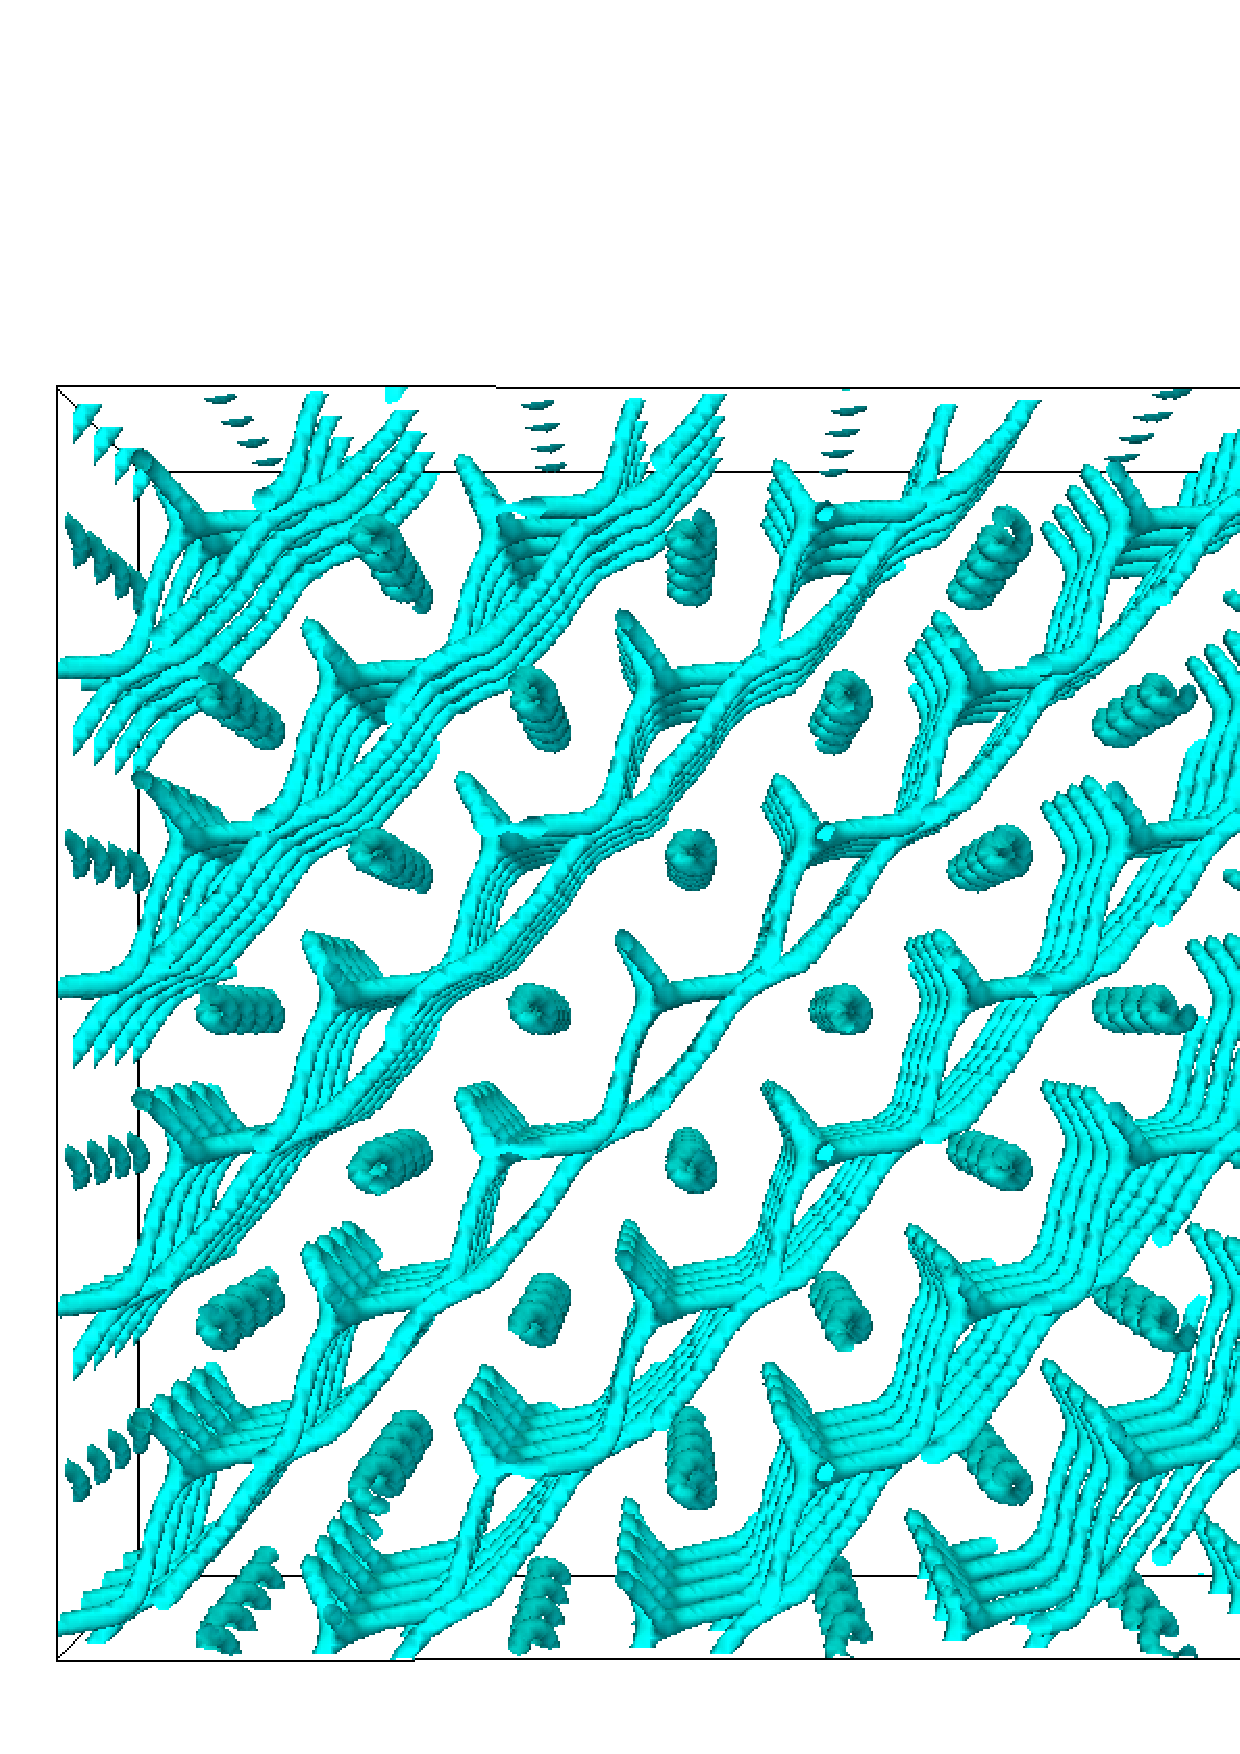
\includegraphics[width=0.32\textwidth]{disc-365k_run914.png}
\includegraphics[width=0.32\textwidth]{disc-367k_run914.png}
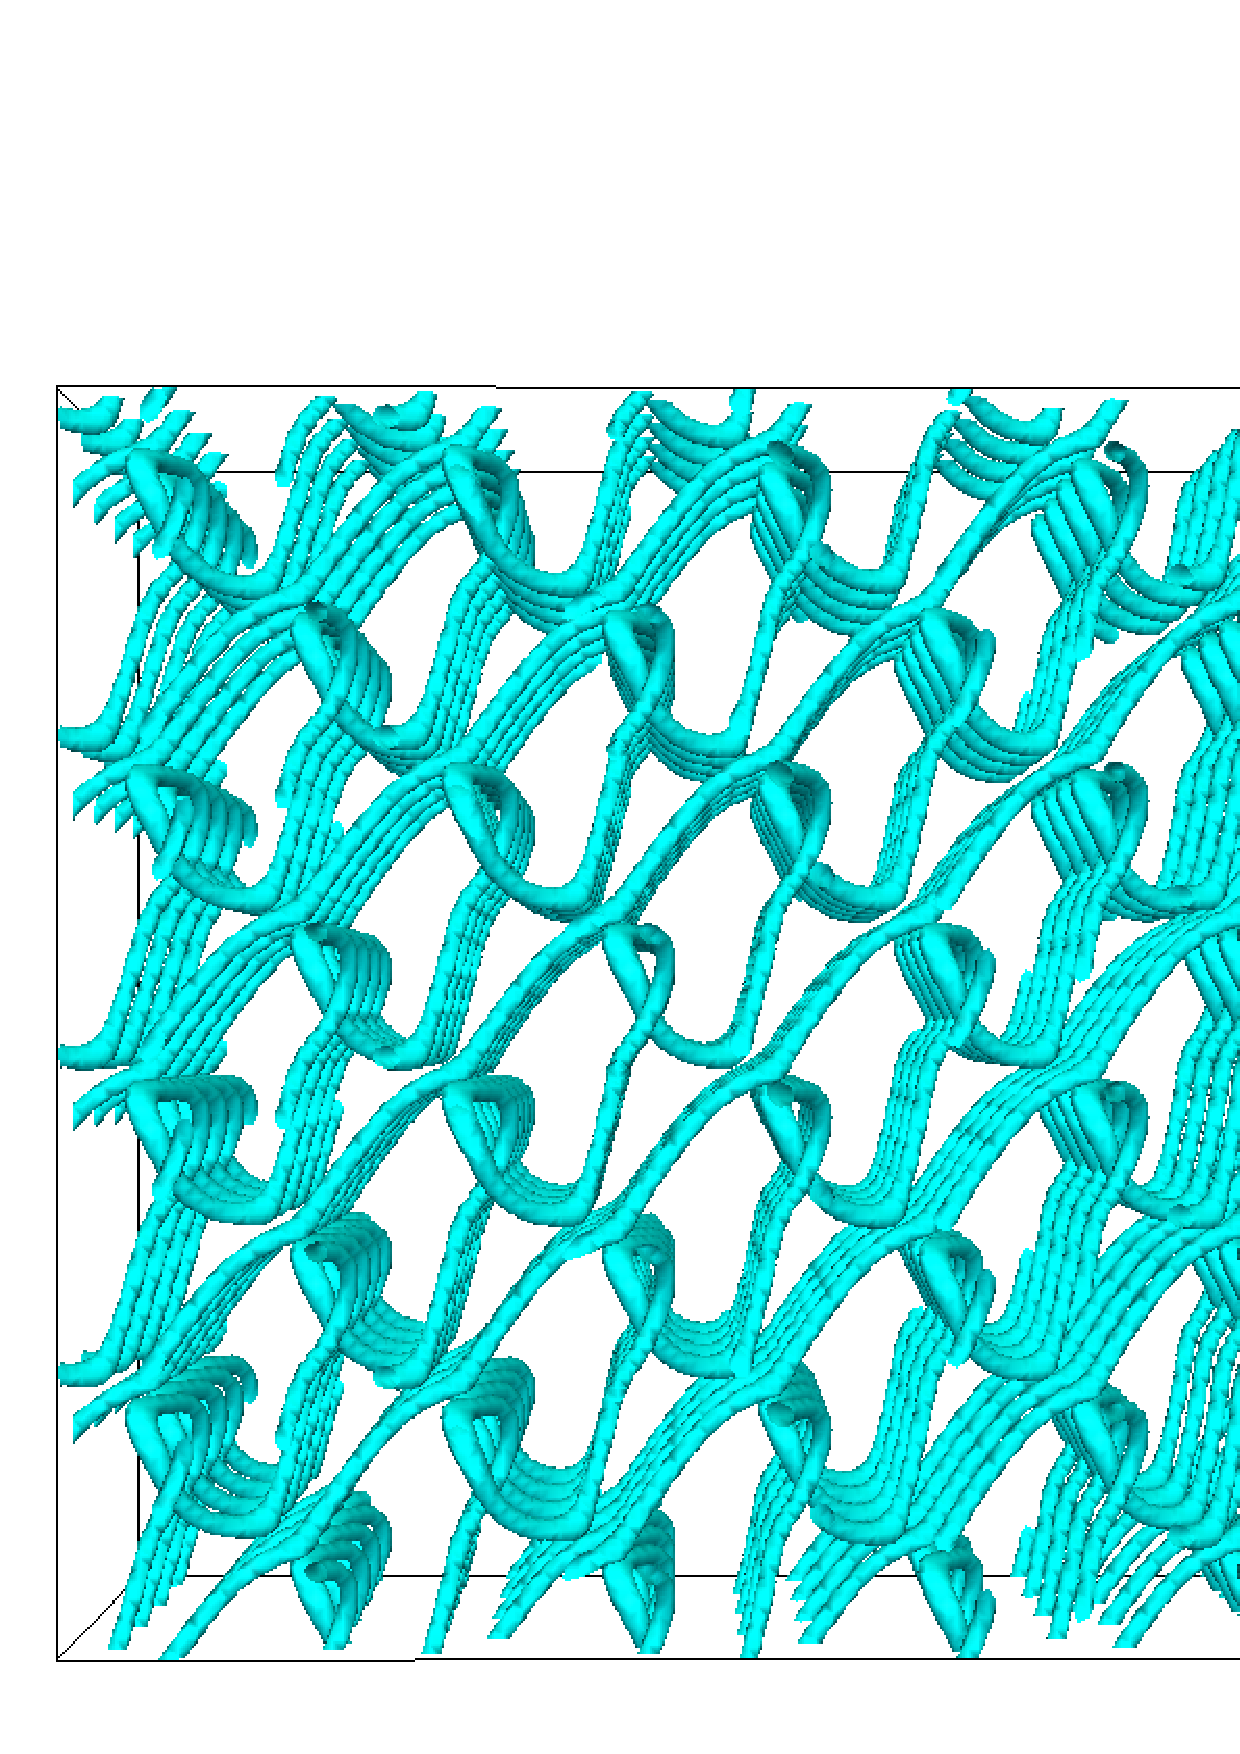
\includegraphics[width=0.32\textwidth]{disc-375k_run914.png}\\
\includegraphics[width=0.32\textwidth]{disc-380k_run914.png}
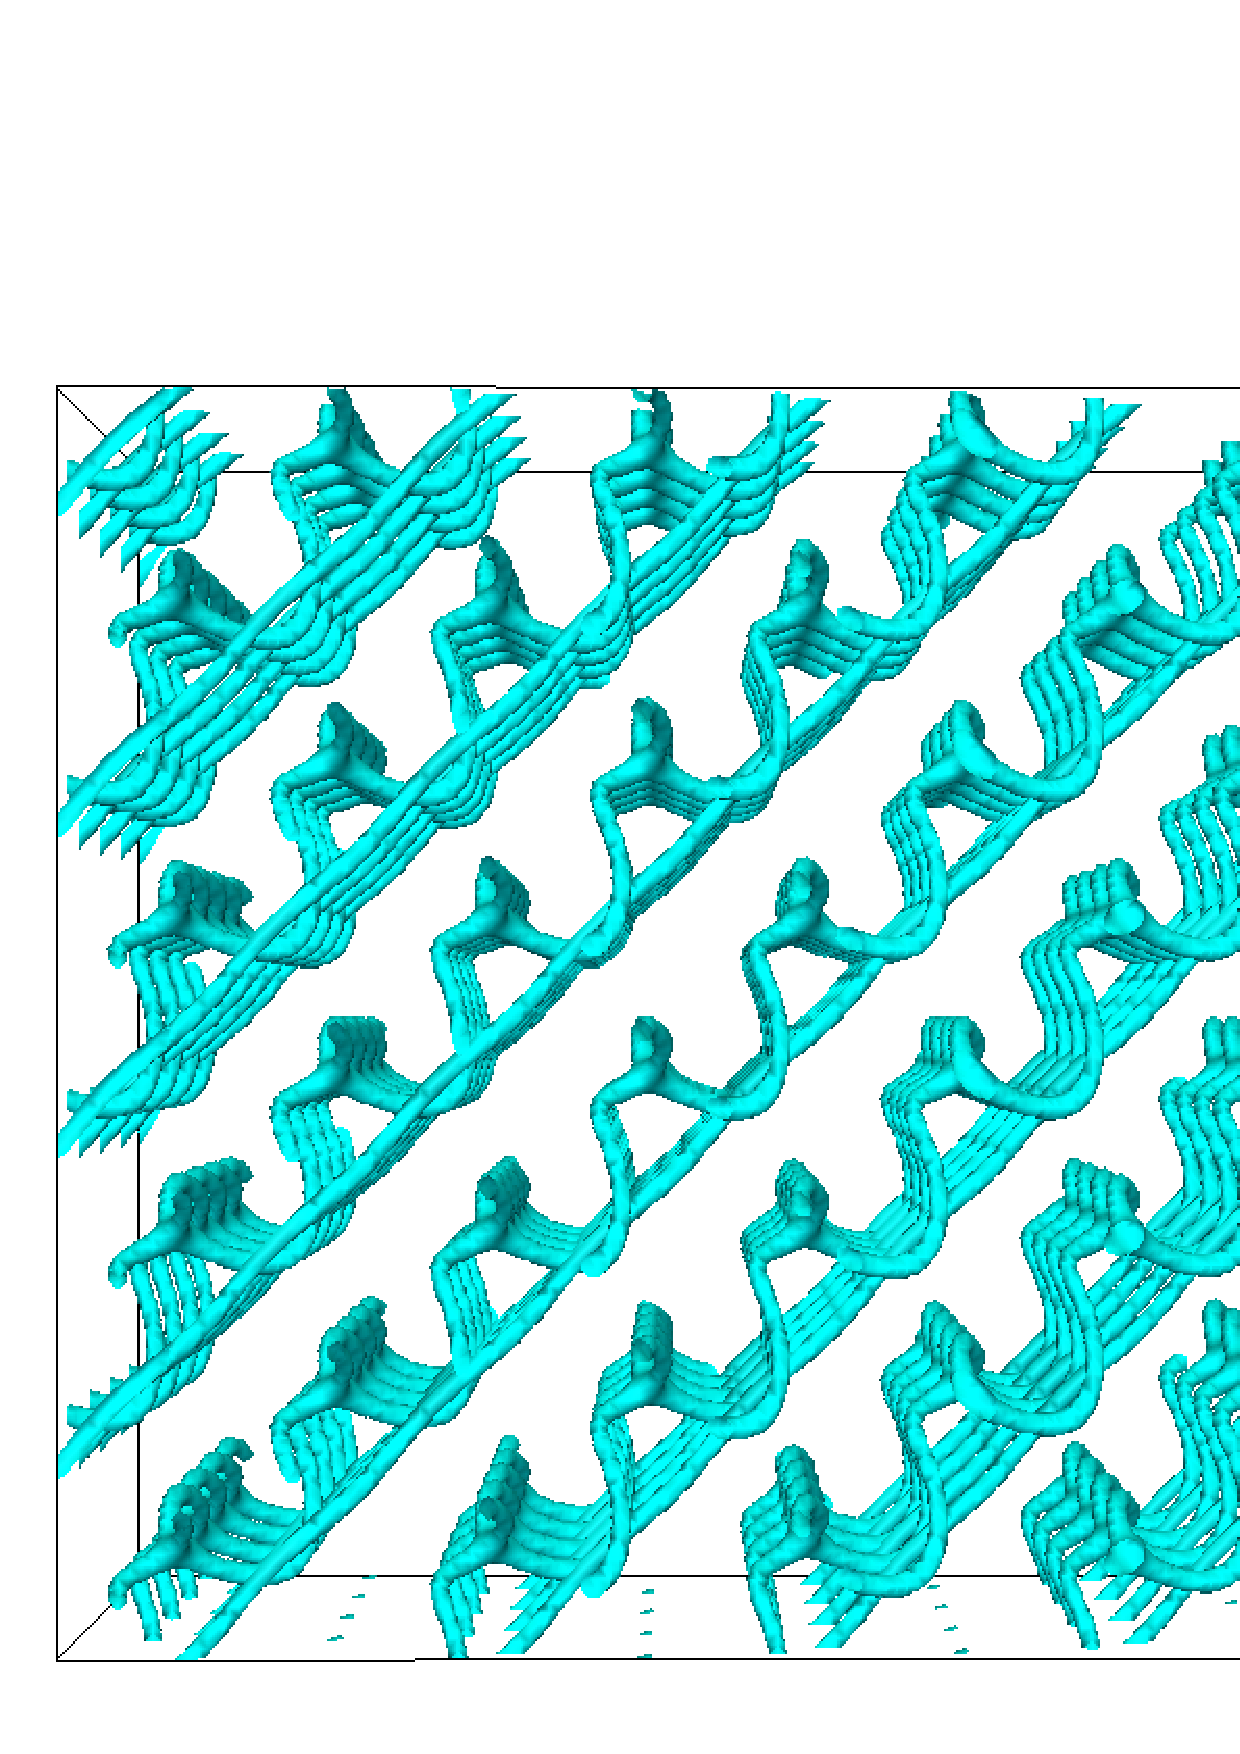
\includegraphics[width=0.32\textwidth]{disc-384k_run914.png}
\includegraphics[width=0.32\textwidth]{disc-389k_run914.png}
\caption{Disclination network of BPI in shear flow: The pictures show a typical sequence of shear-induced transformations in the steady state at $\dot{\gamma}=1.56\e{-4}$ and time steps $t=3.65, 3.67,3.75,3.80,3.84,3.89\e{5}$. The horizontal direction is the vorticity direction, whereas the velocity gradient is oriented along the vertical direction.}
\label{bp1-med}
\end{figure*}

The disclination network and the x- and z-component of the flow velocity are depicted in Fig. \ref{fig7}.
Just as in the previous case of BPII inverting the helix in the initial configuration inverts the sense of motion of the network in z-direction.
Equally it leads to an inversion of the velocities, shown here for a particular time steps, but due to the different topology and the complicated conformational changes there is no simple band structure as previously observed for BPII. 

\begin{figure*}[h]
\includegraphics[width=0.495\textwidth]{v_yz-v_z-360k_run914.png}
\includegraphics[width=0.495\textwidth]{v_yz-v_z-360k_run922.png}
\caption{Velocity patterns in BPI for positive (left) and negative (right) helicity: The pictures show a characteristic time step of the periodically recurring sequence and velocity vectors $(0,v_y,v_z)$ with the component in flow direction set to zero. The colour code gives the magnitude and sign of the z-component. The vertical and horizontal direction are the gradient and vorticity direction, respectivelty. Flow occurs in such a way that the network moves into (out of) the paper plane in the upper (lower) half of the images.}
\label{bp1-velo}
\end{figure*}

Despite qualitative similarities between the BPI and BPII, the quantitative analysis reveals striking differences.
In Fig. \ref{fig8} we show the effective viscosity $\eta_{eff}$ over time and flow curves $\sigma_{chem}(\dot{\gamma})$. 
BPI exhibits pronounced shear-thinning contrary to BPII, whereas the shape of the curves in no longer symmetric.
In fact on approaching the critical shear rate that led in the case of BPII to the disruption of the network, the curves become increasingly complex but remain fully periodic.
The effective viscosity drops by about an order of magnitude between the lowest and the highest shear rates.
Note that the scale has been adapted to allow for the different magnitudes.
The inset can be directly compared with that of Fig. \ref{fig4}.
Interestingly the difference between minima and maxima of the chemical shear stress is much larger than for BPII and for the lowest shear rate we applied the absolute minimum takes even negative values, which are not shown in Fig. \ref{fig4}.
Our understanding of this phenomenon is an interplay of the elastic forces and the individual order paramter configuration of the liquid crystal.
If the system is close to a local minimum of the free energy but moving away from it the increasing strain pumps elastic energy into the system. 
This results in positive chemical stresses as the system tries to withstand the deformation.
However, if the system has sufficiently transformed and is about to overcome a local maximum, it will be pulled towards the next local minumum, which can lead temporarily to negative chemical stresses. 
The inset shows that the chemical stress decreases monotonically with decreasing flow rate, but does not follow a simple power law dependence.

Nevertheless, the disclination network and order parameter strucutre of both phases looks strikingly different in this high flow rate state.
Fig. \ref{fig10} shows a snapshot along the gradient direction and the direction of vorticity.
Contrary to BPII BPI forms rolls which are advected by the flow and undergo a simple affine transformation similar to that of BPII below the break up point.
They meet in $\pm\pi/2$ disclinations, which are oriented along the z-direction.

\begin{figure}[h]
\includegraphics[width=0.32\textwidth]{dir+z-300k_run916.png}
\includegraphics[width=0.32\textwidth]{dir+z-301k_run916.png}
\includegraphics[width=0.32\textwidth]{dir+z-302k_run916.png}
\caption{Director field of BPI at high shear rate: The pictures show a slice of $L_x\times L_y = 64\times64$ lattice sites along the vorticity direction with the flow / gradient direction oriented along the horizontal / vertical axis. The colour code gives the magnitude of the in-plane component of the director field. The data is translationally invariant along the vorticity direction.}
\label{bp1-high}
\end{figure}
 
\begin{figure}[h]
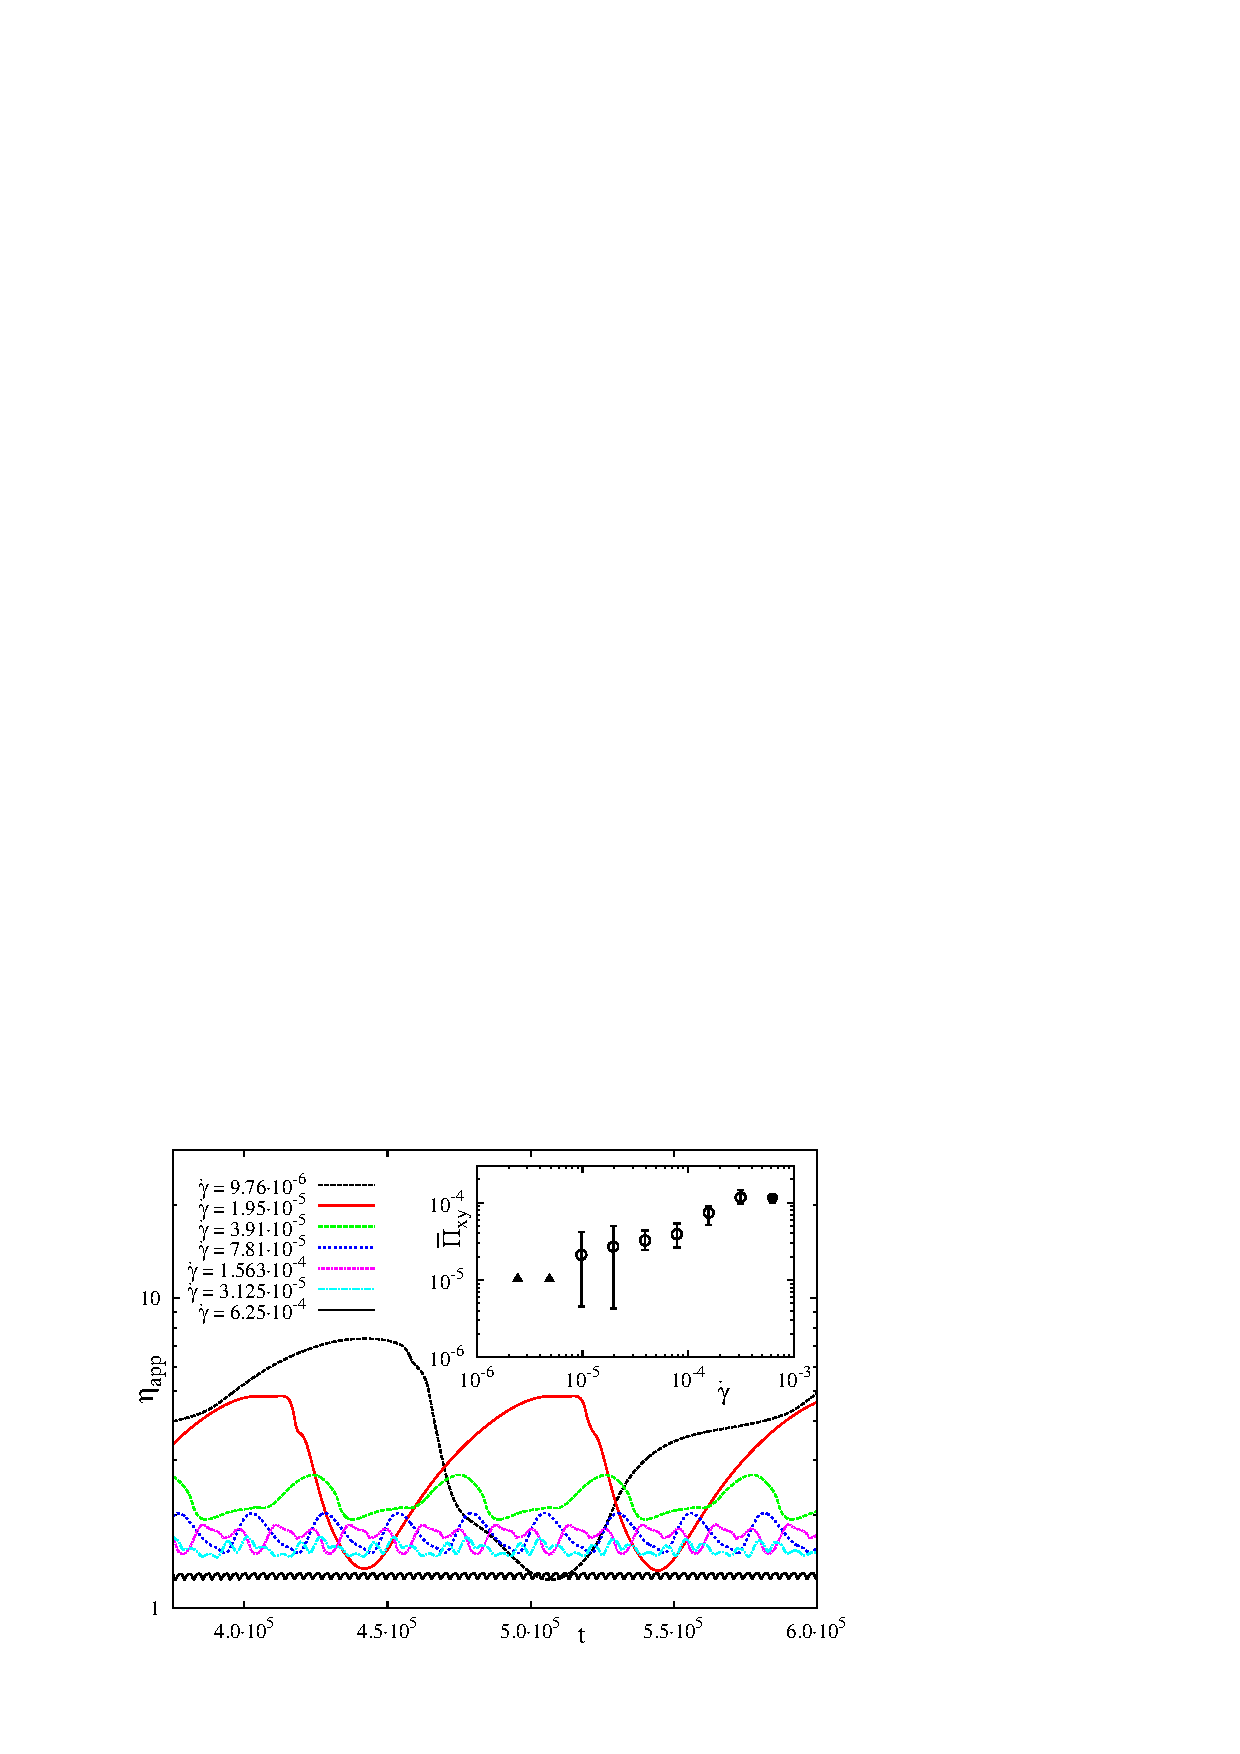
\includegraphics[width=0.495\textwidth]{stress_bp1.pdf}
\includegraphics[width=0.495\textwidth]{stress_vs_strain_bp1.pdf}
\caption{Effective viscosity $\eta_{eff}=\Sigma_{xy}/\dot{\gamma}$ of BPI over time (left) and strain (right). The inset shows the flow curve $\sigma_{chem}(\dot{\gamma})$.}
\label{bp1-rheo}
\end{figure}

A Fourier analysis of the time series of the deviatoric chemical stress $\sigma_{eff,xy}$ or alternatively the free energy density $f$ can provide a further insight into the flow behaviour of BPI.
Fig. \ref{fig9} shows the Fourier spectrum of the time series of the chemical stress.
For simplicity we have always doubled the shear rate, so that the first overtone ocoalesces with the fundamental mode of the next highest shear rate. 
At low shear rates we observe a strong contribution of the first harmonic, which is directly related to the recurrence period $T$, shear rate $\dot{\gamma}$ and unit cell size $l_{u}$ via $\omega_0=2\pi/T=2\pi/(l_{u}\dot{\gamma})$.
The magnitude of higher harmonics decreases monotonously with increasing frequency.
Interestingly the inset of Fig. \ref{fig9} shows that at intermediate shear rates the contribution of higher harmonics becomes more pronounced until after a kind of gap and similar break up the fundamental mode dominates again and the former characteristics are restored.
Remarkably the break up in case of BPI occurs in exactly the same flow rate window as BPII.

\begin{figure}[h]
\includegraphics[width=0.495\textwidth]{stress_bp1_2uc_4uc.pdf}
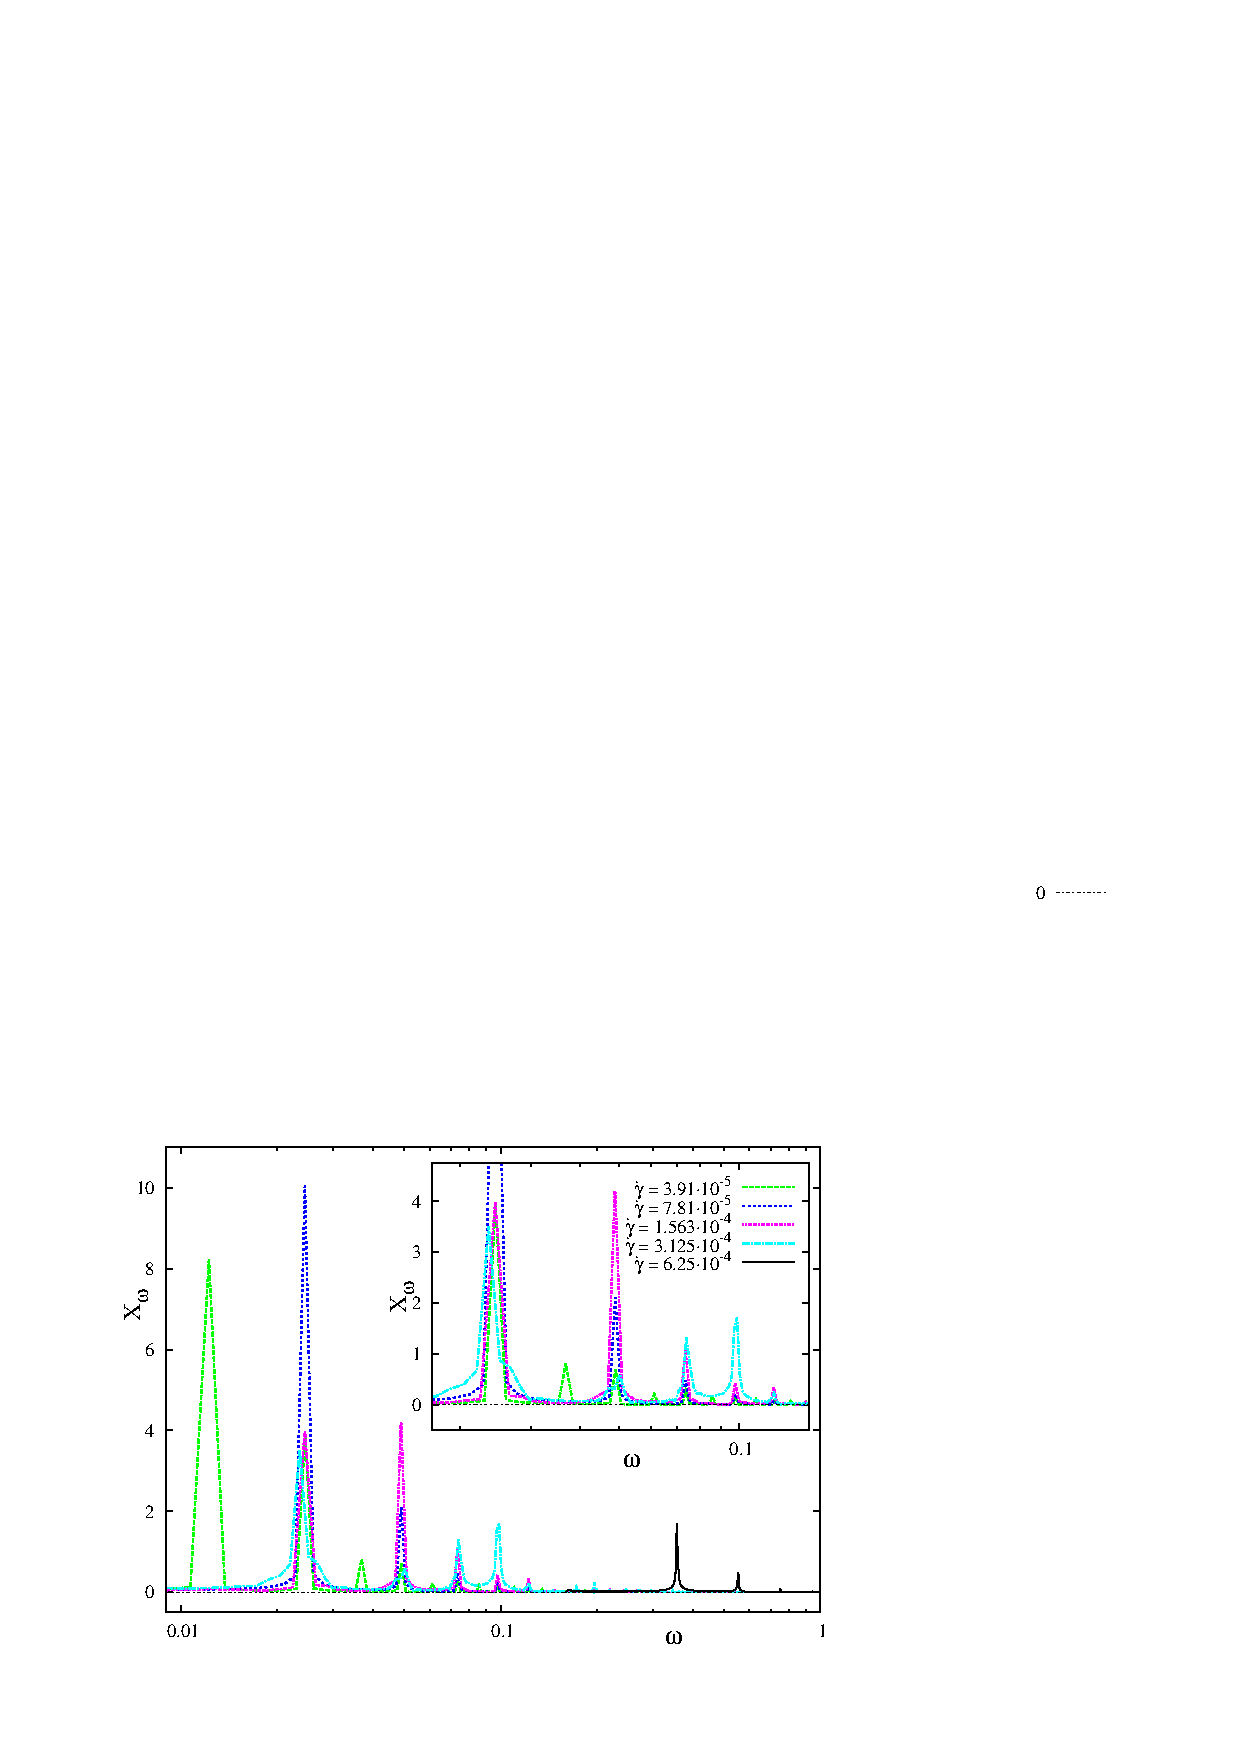
\includegraphics[width=0.495\textwidth]{spectrum_bp1.pdf}
\caption{Spectrum of the time series of the chemical stress over time. The frequency is given in units of $10^2\cdot 2\pi/T$ whereas $T$ is the recurrence period in LB time steps.}
\label{bp1-spec}
\end{figure}


\clearpage

\section{Conclusions}

% If in two-column mode, this environment will change to single-column
% format so that long equations can be displayed. Use
% sparingly.
%\begin{widetext}
% put long equation here
%\end{widetext}

% figures should be put into the text as floats.
% Use the graphics or graphicx packages (distributed with LaTeX2e)
% and the \includegraphics macro defined in those packages.
% See the LaTeX Graphics Companion by Michel Goosens, Sebastian Rahtz,
% and Frank Mittelbach for instance.
%
% Here is an example of the general form of a figure:
% Fill in the caption in the braces of the \caption{} command. Put the label
% that you will use with \ref{} command in the braces of the \label{} command.
% Use the figure* environment if the figure should span across the
% entire page. There is no need to do explicit centering.

% \begin{figure}
% \includegraphics{}%
% \caption{\label{}}
% \end{figure}

% Surround figure environment with turnpage environment for landscape
% figure
% \begin{turnpage}
% \begin{figure}
% \includegraphics{}%
% \caption{\label{}}
% \end{figure}
% \end{turnpage}

% tables should appear as floats within the text
%
% Here is an example of the general form of a table:
% Fill in the caption in the braces of the \caption{} command. Put the label
% that you will use with \ref{} command in the braces of the \label{} command.
% Insert the column specifiers (l, r, c, d, etc.) in the empty braces of the
% \begin{tabular}{} command.
% The ruledtabular enviroment adds doubled rules to table and sets a
% reasonable default table settings.
% Use the table* environment to get a full-width table in two-column
% Add \usepackage{longtable} and the longtable (or longtable*}
% environment for nicely formatted long tables. Or use the the [H]
% placement option to break a long table (with less control than 
% in longtable).
% \begin{table}%[H] add [H] placement to break table across pages
% \caption{\label{}}
% \begin{ruledtabular}
% \begin{tabular}{}
% Lines of table here ending with \\
% \end{tabular}
% \end{ruledtabular}
% \end{table}

% Surround table environment with turnpage environment for landscape
% table
% \begin{turnpage}
% \begin{table}
% \caption{\label{}}
% \begin{ruledtabular}
% \begin{tabular}{}
% \end{tabular}
% \end{ruledtabular}
% \end{table}
% \end{turnpage}

% Specify following sections are appendices. Use \appendix* if there
% only one appendix.
\appendix*

\begin{table*}
\begin{tabular}{|c|| c || c |c |c||c| c| c||c| c| c|}
\hline
$\dot{\gamma}$ & $q_0$ & $\bar{v}_{x,min}$ & $\bar{v}_{x,max}$ & $\bar{v}_{x,std}$ & $\bar{v}_{y,min}$ & $\bar{v}_{y,max}$ & $\bar{v}_{y,std}$ & $\bar{v}_{z,min}$ & $\bar{v}_{z,max}$ & $\bar{v}_{z,std}$ \\
\hline
BPI \\
\hline
0.244 & 0.1388 &-15.79 &15.57 &1.04 &-0.89 &0.91 &0.95 &-1.59 &1.19 &1.27 \\
0.488 &0.1388 &-31.11 &31.25 &1.31 &-0.93 &0.98 &1.28 &-1.62 &1.10 &1.40 \\
0.976 &0.1388 &-62.24 &62.37 &2.51 &-1.31 &1.25 &2.68 &-1.24 &0.87 &2.65 \\
1.95 & 0.1388 &-124.65 &124.82 &3.62&  -2.49 &2.50 &4.51 &-1.89 & 1.62 &3.51 \\
3.91 &0.1388 &-248.69 &248.74 &3.90&  -3.31 &3.35 &4.21 &-2.56 & 2.88 &4.39 \\
7.81 &0.1388 &-497.22 &496.16 &4.46 &-6.49 &6.56 &7.99 &-5.31 & 7.46 &6.81 \\ 
15.63 &0.1388 &-992.46 &993.18 &10.36 &-3.08 &3.17 &10.49 &\bf{-2.87} & \bf{3.57} &10.54 \\
15.63 &-0.1388 &-992.46 &993.18 &10.36 &-3.08 &3.17 &10.49 &\bf{-3.57} & \bf{2.87} &10.54 \\
31.25 &0.1388 & -1988.36 &1986.71 &16.85 &-4.08 &4.46 &15.94 &-11.37 & 12.16 &19.38\\
62.50 &0.1388 & -4039.41 &3995.3  & 20.57 & -62.63 & 62.13 & 24.68 &-73.52 & 110.76 & 33.26 \\
\hline
BPII \\
\hline
0.244 &0.1963 &-7.75 &7.70 &0.13 &-0.17 &0.17 &0.13 &-0.24 &0.23 &0.19 \\
0.488 &0.1963 &-15.50 &15.40 &0.19 &-0.32 &0.30 &0.21 &-0.43 &0.42 &0.29 \\
0.976 &0.1963 &-31.01 &30.80 &0.33 &-0.60 &0.58 &0.41 &-0.85 &0.79 &0.47 \\
1.95 & 0.1963 &-62.04  &61.60 & 0.97 & -1.09 &1.07 & 0.76 & -1.64 & 1.55 & 0.81\\
3.91 & 0.1963 &-123.93 &123.18 & 1.76 &-1.66 &1.70 & 1.45 &-3.09& 2.73 &1.47\\
7.81 &0.1963  &-247.67 &246.45 & 3.20 &-2.62 &2.71 & 2.67 &-5.78 & 4.77 &2.74\\
15.63 &0.1963 &-494.85 &493.09 & 5.64 &-3.13 &3.31 &4.24 &\bf{-10.00} & \bf{7.66} &4.33\\
15.63 &-0.1963&-494.85 &493.09 & 5.64 & -3.13 &3.31 &4.24 &\bf{-7.66} & \bf{10.00} &4.33\\
31.25 &0.1963 &-988.73 &985.93 &8.96  &-1.79 &1.82 &5.86 &-14.39 & 11.04 &6.35\\
62.50 &0.1963 & -1969.41  & 1969.41 & 3.07 & -1.20 & 1.20 & 0.38 &-0.96 & 1.48 &0.38 \\
\hline
\end{tabular}
\caption{Time-averaged velocity components in shear flow for BPI ($\tau=-0.5, \kappa=1.0$) and BPII ($\tau=-0.5, \kappa=2.0$): Given are minumum and maximum values in $10^{-5}$ lattice units and the maximum standard deviation over the entire time sequence excluding transient dynamics, which means times t$\ge 200000$ for BPI and t$\ge 30000$ in case of BPII.
\label{tab1}}
\end{table*}
%\section{}

% If you have acknowledgments, this puts in the proper section head.
\begin{acknowledgments}
Thanks folks!
\end{acknowledgments}

% Create the reference section using BibTeX:
\bibliography{bprheo}

\end{document}
%
% ****** End of file apstemplate.tex ******

